\documentclass[11pt,a4paper]{article}
\usepackage[utf8]{inputenc}
\usepackage[T1]{fontenc}
\usepackage[norsk]{babel}
\usepackage{tgtermes}
\usepackage{tgheros}
\renewcommand{\ttdefault}{txtt}
\usepackage{amsmath,amssymb}
\usepackage[a4paper,left=2.45cm,right=2.6cm,top=2.3cm,bottom=2.2cm,headsep=0.9cm]{geometry}
\usepackage{fancyhdr}
\usepackage{lastpage}
\usepackage{xcolor}
\usepackage{tikz}
\usepackage{pgfplots}
\pgfplotsset{compat=1.18}
\usepackage{booktabs}
\usepackage{array}
\usepackage{enumitem}
\usepackage{listings}
\usepackage{needspace}
\usepackage{multirow}
\usetikzlibrary{positioning,arrows.meta,calc}
\definecolor{insgrey}{gray}{0.42}
\definecolor{radiogrey}{gray}{0.70}
\setlength{\parindent}{0pt}
\setlength{\parskip}{0.45em}
\setlist[itemize]{itemsep=0pt,topsep=2pt,label=\textbullet,font=\sffamily}
\lstset{basicstyle=\ttfamily\small,columns=fullflexible,keepspaces=true,
  showstringspaces=false,upquote=true,aboveskip=0.6em,belowskip=0.6em,
  literate={æ}{{\ae}}1 {ø}{{\o}}1 {å}{{\aa}}1 {Æ}{{\AE}}1 {Ø}{{\O}}1 {Å}{{\AA}}1}
\pagestyle{fancy}
\fancyhf{}
\renewcommand{\headrulewidth}{0pt}
\fancyhead[R]{\fontsize{7.5}{9}\selectfont\sffamily\color{insgrey}TDT4172 - Introduksjon til maskinlæring - Øvingssett 6}
\fancyfoot[R]{\fontsize{7}{9}\selectfont\sffamily\color{insgrey}\thepage/\pageref{LastPage}}
\newcommand{\delstart}[1]{\clearpage
  \noindent\hspace*{-1.55em}\makebox[1.55em][l]{\sffamily\bfseries\fontsize{12}{14}\selectfont\raisebox{0.35em}{#1}}%
  {\sffamily\bfseries\fontsize{18}{22}\selectfont Part #1}\par\vspace{1.0em}}
\newcommand{\sporsmal}[1]{\par\Needspace{9\baselineskip}\vspace{1.9em}%
  \noindent{\bfseries Spørsmål #1}\par\vspace{-0.45em}%
  \noindent{\bfseries -{}-{}-{}-{}-{}-{}-{}-{}-{}-{}-{}-{}-{}-{}-{}-{}-}\par\vspace{-0.15em}}
\newcommand{\velg}[1]{\par\Needspace{6\baselineskip}\noindent{\bfseries #1}\par\vspace{0.3em}}
\newcommand{\radio}[1]{\tikz[baseline=-0.62ex]{\draw[radiogrey,line width=0.45pt,fill=gray!5] (0,0) circle (0.56em);
  \node[inner sep=0pt,font=\sffamily\fontsize{5.5}{6}\selectfont,text=insgrey] at (0,0) {#1};}}
\newenvironment{alternativer}{\begin{list}{}{\setlength{\leftmargin}{2.35em}\setlength{\labelwidth}{1.4em}%
  \setlength{\labelsep}{0.6em}\setlength{\itemsep}{0.85em}\setlength{\topsep}{0.45em}\setlength{\parsep}{0pt}}%
  \sffamily\fontsize{10}{12.6}\selectfont}{\end{list}}
\newcommand{\alt}[2]{\item[\radio{#1}]#2}
\newcommand{\makspoeng}{\par\vspace{2.2em}\hfill{\sffamily\fontsize{8.5}{10}\selectfont Maks poeng: 10}\hspace*{0.5em}\par}
\begin{document}

\noindent\hspace*{-1.55em}\makebox[1.55em][l]{\raisebox{0.3em}{\sffamily\bfseries\fontsize{11}{12}\selectfont i}}%
{\sffamily\bfseries\fontsize{18}{22}\selectfont Frontpage}\par\vspace{1.1em}

{\bfseries Eksamensoppgave i TDT4172 - Introduksjon til maskinlæring}\\
{\bfseries Øvingssett:} 6 av 10 (uoffisielt øvingssett)\\
{\bfseries Tid:} 4 timer

\vspace{0.6em}
{\bfseries Faglig kontakt:} --- (øvingssett, ikke en offisiell eksamen)\\
{\bfseries Møter i eksamenslokalet:} Nei

\vspace{0.6em}
{\bfseries Hjelpemiddelkode/Tillatte hjelpemidler:} D / Ingen trykte eller håndskrevne hjelpemidler tillatt.
Bestemt, enkel kalkulator tillatt.

\vspace{0.6em}
{\bfseries\underline{ANNEN INFORMASJON:}}

\vspace{0.4em}
{\bfseries Les oppgavene nøye og gjør dine egne antagelser.} Presiser i besvarelsen hvilke forutsetninger du
har lagt til grunn i tolkning/avgrensing av oppgaven.

Dette øvingssettet er laget for egentrening, med samme format og vanskelighetsgrad som de
siste ordinære eksamenene i emnet. Løsningsforslaget står på siste side.

\vspace{1.6em}
{\bfseries\underline{FAGSPESIFIKK INFORMASJON}}

\vspace{0.4em}
{\bfseries Ingen papirhåndtegninger:}\\
Denne eksamenen tillater ikke bruk av håndtegninger.

\vspace{1.4em}
{\bfseries Vekting av oppgavene}:\\
Denne eksamenen inneholder flervalgsoppgaver organisert i ti grupper på fire spørsmål hver. Hver
gruppe vurderes separat etter følgende regler:

\vspace{0.6em}
For hver av de fire spørsmålene i gruppen får du følgende poeng
\begin{itemize}[leftmargin=2.2em,label=\textperiodcentered,itemsep=0pt]
\item {\bfseries Riktig svar:} +2,5 poeng
\item {\bfseries Feil svar (et alternativ er valgt, men ikke korrekt):} $-$0,83 poeng
\item {\bfseries Ikke besvart:} 0 poeng
\end{itemize}
{\bfseries Merk} at dersom du først har valgt et svaralternativ, kan du {\bfseries ikke velge det bort} igjen. Da må du
svare på det spørsmålet. Med andre ord mister du muligheten til å la et spørsmål stå blankt så fort
du har trykket på et alternativ.

\vspace{0.6em}
Poengsummen for hver gruppe er {\bfseries summen} av poengene for de fire enkeltspørsmålene.\\
For {\bfseries alle spørsmålene} gjelder en {\bfseries null-grense}: dersom summen for denne gruppen blir negativ,
settes verdien til {\bfseries 0}. Den totale poengsummen på eksamen er summen av poengene fra alle
gruppene.

\delstart{1}
\sporsmal{1}
For ett datapunkt er gradienten av cross-entropy loss med hensyn på $w_1$ lik $(\hat y - y)\,x_1$.
Tabellen viser fire treningspunkter og modellens nåværende prediksjoner.
\begin{center}
\begin{tabular}{lcccc}
\toprule
Punkt & P1 & P2 & P3 & P4\\
\midrule
$x_1$ & 1.0 & 0.5 & 2.0 & $-3.0$\\
$y$ & 1 & 0 & 1 & 0\\
$\hat y$ & 0.95 & 0.90 & 0.70 & 0.12\\
\bottomrule
\end{tabular}
\end{center}
Hvilket punkt gir det største bidraget (i absoluttverdi) til $\partial L/\partial w_1$?
\velg{Velg ett alternativ:}
\begin{alternativer}
\alt{A}{Alle fire bidrar like mye, siden gradienten er et gjennomsnitt over treningspunktene}
\alt{B}{P3, fordi produktet av avviket $\hat y - y$ og verdien $x_1$ er størst i absoluttverdi der}
\alt{C}{P2, fordi det er punktet der prediksjonen $\hat y$ ligger lengst unna sin label $y$}
\alt{D}{P4, fordi det er punktet med den største absoluttverdien av featuren $x_1$}
\end{alternativer}
\sporsmal{2}
Figuren viser tap (loss) og accuracy på \textbf{treningsdataene} etter hver epoke for en logistisk
regresjonsmodell som er trent i 30 epoker.
\begin{center}
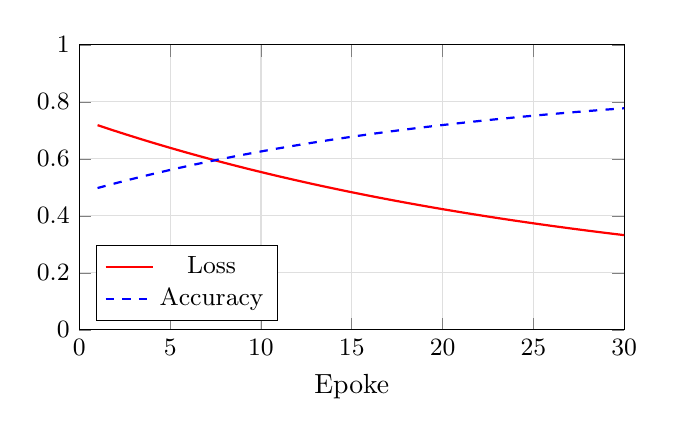
\begin{tikzpicture}
\begin{axis}[width=8.5cm,height=5.2cm,xmin=0,xmax=30,ymin=0,ymax=1,
  xlabel={Epoke},grid=major,grid style={gray!25},legend pos=south west,
  legend style={font=\small},tick label style={font=\small}]
\addplot[thick,red,domain=1:30,samples=60] {0.62*exp(-x/28)+0.12};
\addlegendentry{Loss}
\addplot[thick,blue,dashed,domain=1:30,samples=60] {0.88-0.40*exp(-x/22)};
\addlegendentry{Accuracy}
\end{axis}
\end{tikzpicture}
\end{center}

Hva er den beste tolkningen av kurvene?
\velg{Velg ett alternativ:}
\begin{alternativer}
\alt{A}{Læringsraten er for høy, siden tapet fortsatt endrer seg mye mellom de siste epokene}
\alt{B}{Modellen har konvergert, siden accuracy har passert 0.7 og tapet er under 0.4}
\alt{C}{Modellen er ikke ferdig trent; kurvene har ikke flatet ut, så den bør trenes lenger}
\alt{D}{Modellen overtilpasser, siden tapet på treningsdataene fortsatt minker etter 30 epoker}
\end{alternativer}
\sporsmal{3}
Tabellen viser et lite datasett der \emph{Mislighold} er target (tom celle = manglende verdi).
\begin{center}
\begin{tabular}{rlrrlc}
\toprule
KundeID & Navn & Alder & Inntekt & Sivilstatus & Mislighold \\
\midrule
1001 & Hansen & 34 & 520 & gift & 0 \\
1002 &        & 51 & 610 & ugift & 0 \\
1003 & Berg   & 27 & 380 & ugift & 1 \\
1004 & Lie    &    & 450 & gift & 0 \\
1005 & Dahl   & 45 & 700 & skilt & 0 \\
1006 & Moe    & 38 &     & gift & 1 \\
1007 & Bakke  & 62 & 590 & ugift & 0 \\
\bottomrule
\end{tabular}
\end{center}
Du fjerner først kolonnene som ikke bør brukes som features, og kjører deretter \texttt{df.dropna()}.

Hvor mange rader og hvor mange features (target ikke medregnet) står du igjen med?
\velg{Velg ett alternativ:}
\begin{alternativer}
\alt{A}{4 rader og 5 features}
\alt{B}{4 rader og 3 features}
\alt{C}{5 rader og 3 features}
\alt{D}{7 rader og 4 features}
\end{alternativer}
\sporsmal{4}
Feature \emph{Alder} skaleres med \texttt{MinMaxScaler}, som tilpasses (\texttt{fit}) på treningsdataene.
I treningsdataene er minste alder 20 og største 60. Testsettet inneholder en person på 70 år.

Hvilken verdi gir \texttt{scaler.transform} for denne personen?
\velg{Velg ett alternativ:}
\begin{alternativer}
\alt{A}{$0.83$}
\alt{B}{$1.25$}
\alt{C}{$0.71$}
\alt{D}{$1.00$}
\end{alternativer}
\makspoeng

\delstart{2}
\sporsmal{1}
Et treningssett har 5000 normale produkter og 250 defekte. Du bruker \textbf{random oversampling}
av minoritetsklassen til klassene er like store.

Hva blir størrelsen på treningssettet, og hva er den viktigste risikoen?
\velg{Velg ett alternativ:}
\begin{alternativer}
\alt{A}{$10\,000$ punkter; mange identiske kopier av minoritetspunktene kan gi overtilpasning}
\alt{B}{$500$ punkter; det blir få datapunkter totalt, og modellen kan derfor undertilpasse}
\alt{C}{$9\,750$ punkter; nye syntetiske defekte produkter gjør modellen mer robust mot støy}
\alt{D}{$5\,250$ punkter; datasettet er uendret, men de defekte produktene får høyere vekt i tapet}
\end{alternativer}
\sporsmal{2}
Du trener med vektet binary cross-entropy
\[
L = -w_1\, y \ln \hat{y} - w_0\,(1-y)\ln(1-\hat{y}),
\]
med $w_0 = 1$ og $w_1 = 5$ for den underrepresenterte klassen 1, på det opprinnelige treningssettet.

Hvilken annen fremgangsmåte gir omtrent samme totale tap som modellen minimerer under trening?
\velg{Velg ett alternativ:}
\begin{alternativer}
\alt{A}{Å trene med uvektet tap og deretter gange alle de lærte vektene $\mathbf{w}$ med 5}
\alt{B}{Å trene med uvektet tap og deretter senke klassifiseringsterskelen fra 0.5 til 0.2}
\alt{C}{Å gange feature-verdiene til punktene i klasse 1 med 5 og trene med uvektet tap}
\alt{D}{Å la hvert punkt i klasse 1 forekomme fem ganger og trene med uvektet tap}
\end{alternativer}
\sporsmal{3}
En klassifikator gir disse skårene på seks testpunkter:
\begin{center}
\begin{tabular}{lccc}
\toprule
Positive punkter & 0.9 & 0.7 & 0.4 \\
Negative punkter & 0.8 & 0.3 & 0.2 \\
\bottomrule
\end{tabular}
\end{center}
ROC AUC kan tolkes som sannsynligheten for at et tilfeldig valgt positivt punkt får høyere skår enn et
tilfeldig valgt negativt punkt.

Hva er ROC AUC for disse punktene?
\velg{Velg ett alternativ:}
\begin{alternativer}
\alt{A}{$0.22$}
\alt{B}{$0.33$}
\alt{C}{$0.78$}
\alt{D}{$0.67$}
\end{alternativer}
\sporsmal{4}
En svindelmodell evalueres på 10\,000 transaksjoner, hvorav 50 er svindel. Modellen finner 20 av
svindeltilfellene og gir 30 falske alarmer. En kollega regner ut precision og recall med
\emph{normal transaksjon} som positiv klasse, og får begge til omtrent $0.997$.

Hvilket utsagn er riktig?
\velg{Velg ett alternativ:}
\begin{alternativer}
\alt{A}{Tallene blir de samme uansett hvilken klasse som regnes som positiv, så modellen finner svindel godt}
\alt{B}{Med svindel som positiv klasse blir både precision og recall 0.40, så tallene skjuler en svak modell}
\alt{C}{Med svindel som positiv klasse blir begge 0.003, siden metrikkene da er 1 minus kollegaens verdier}
\alt{D}{Med svindel som positiv klasse blir recall 0.40, men precision er fortsatt 0.997, siden alarmene er få}
\end{alternativer}
\makspoeng

\delstart{3}
\sporsmal{1}
Et beslutningstre bygges etter pseudokoden fra forelesningen. En node splittes på den kategoriske
featuren \emph{Embarked}, med én gren for hver av verdiene C, Q og S. Noden inneholder 12 treningspunkter,
hvorav 8 overlevde og 4 omkom, men \textbf{ingen} av dem har \emph{Embarked} $=$ Q.
Treet har ikke nådd \texttt{max\_depth}, og det finnes fortsatt features å splitte på.

Hva predikerer grenen for Q?
\velg{Velg ett alternativ:}
\begin{alternativer}
\alt{A}{Omkom, siden en partisjon uten data får klasse 0 når $p/(p+n)$ ikke kan beregnes}
\alt{B}{Majoritetsklassen i hele treningssettet, siden grenen ikke har egne datapunkter}
\alt{C}{Ingen klasse; grenen fjernes, og punkter med Q sendes videre til den største grenen}
\alt{D}{Overlevde, siden en partisjon uten data får den dominerende klassen i foreldrenoden}
\end{alternativer}
\sporsmal{2}
Et beslutningstre med begrenset dybde har en løvnode som inneholder 7 treningspunkter fra klasse A og
3 fra klasse B. Treet bruker \textbf{majoritetsregelen} i løvnodene.

Hvilket utsagn er riktig?
\velg{Velg ett alternativ:}
\begin{alternativer}
\alt{A}{Hvert punkt som havner i noden, får klassen til det nærmeste av de 10 treningspunktene i noden}
\alt{B}{Hvert punkt som havner i noden, får A med sannsynlighet 0.7 og B med 0.3, trukket tilfeldig ved prediksjon}
\alt{C}{Alle punkter i noden predikeres som A, og treningsfeilen der er Gini-urenheten $1 - 0.7^2 - 0.3^2 = 0.42$}
\alt{D}{Alle punkter i noden predikeres som A, så 3 av de 10 treningspunktene der blir feilklassifisert}
\end{alternativer}
\sporsmal{3}
For et datapunkt $\mathbf{x}$ og to klasser har en modell estimert
\[
p(C_1) = 0.3,\quad p(\mathbf{x}\mid C_1) = 0.20, \qquad p(C_0) = 0.7,\quad p(\mathbf{x}\mid C_0) = 0.05 .
\]

Hvilket utsagn er riktig?
\velg{Velg ett alternativ:}
\begin{alternativer}
\alt{A}{Klasse 1 velges; evidensen $p(\mathbf{x})$ er lik for begge klasser og trengs ikke for å finne argmax}
\alt{B}{Klasse 0 velges, fordi likelihooden $p(\mathbf{x}\mid C_0)$ er minst og dermed gir minst tap}
\alt{C}{Klasse 1 velges, men først etter at evidensen $p(\mathbf{x})$ er beregnet, siden den er ulik for de to klassene}
\alt{D}{Klasse 0 velges, fordi prioren $p(C_0) = 0.7$ er størst og derfor dominerer posterior}
\end{alternativer}
\sporsmal{4}
Et datasett med 20 e-poster har 5 spam og 15 ikke spam. Tellingene for to binære features er:
\begin{center}
\begin{tabular}{lcc}
\toprule
 & Spam (5) & Ikke spam (15) \\
\midrule
Inneholder ordet ``gratis'' & 4 & 3 \\
Inneholder en lenke & 4 & 6 \\
\bottomrule
\end{tabular}
\end{center}
En ny e-post inneholder ordet ``gratis'', men \emph{ingen} lenke. Bruk Naive Bayes med skåren
$p(C)\prod_i p(x_i\mid C)$.

Hva blir klassifiseringen og de to skårene?
\velg{Velg ett alternativ:}
\begin{alternativer}
\alt{A}{Ikke spam, med skår 0.01 for spam og 0.36 for ikke spam}
\alt{B}{Spam, med skår 0.16 for spam og 0.12 for ikke spam}
\alt{C}{Spam, med skår 0.16 for spam og 0.06 for ikke spam}
\alt{D}{Ikke spam, med skår 0.04 for spam og 0.09 for ikke spam}
\end{alternativer}
\makspoeng

\delstart{4}
\sporsmal{1}
Du har et datasett med $n = 500$ punkter og vurderer \textbf{leave-one-out-kryssvalidering} (LOOCV)
mot \textbf{10-fold kryssvalidering}.

Hvilket utsagn er riktig?
\velg{Velg ett alternativ:}
\begin{alternativer}
\alt{A}{LOOCV krever bare én trening, siden den samme modellen evalueres på hvert enkelt punkt etter tur}
\alt{B}{LOOCV og 10-fold krever like mange treninger, men LOOCV har et mindre valideringssett i hver iterasjon}
\alt{C}{LOOCV krever 500 treninger med ett utelatt punkt hver gang, mens 10-fold bare krever 10 treninger}
\alt{D}{10-fold bruker flere punkter til trening i hver iterasjon enn LOOCV, og gir derfor et bedre estimat}
\end{alternativer}
\sporsmal{2}
Et nevralt nettverk trenes med \textbf{early stopping}: treningen stoppes når valideringstapet ikke har
blitt lavere enn sitt hittil beste på 3 epoker på rad.
\begin{center}
\small
\begin{tabular}{lcccccccccccc}
\toprule
Epoke & 1 & 2 & 3 & 4 & 5 & 6 & 7 & 8 & 9 & 10 & 11 & 12 \\
\midrule
Treningstap & .95 & .74 & .61 & .53 & .47 & .42 & .38 & .35 & .32 & .30 & .28 & .26 \\
Valideringstap & .90 & .70 & .58 & .52 & .50 & .49 & .495 & .51 & .50 & .52 & .54 & .56 \\
\bottomrule
\end{tabular}
\end{center}

Etter hvilken epoke stopper treningen?
\velg{Velg ett alternativ:}
\begin{alternativer}
\alt{A}{Epoke 6}
\alt{B}{Epoke 7}
\alt{C}{Epoke 8}
\alt{D}{Epoke 9}
\end{alternativer}
\sporsmal{3}
Modellen $f(x) = \beta_0 + \beta_1 x$ med $\beta_0 = 1$ og $\beta_1 = 1.5$ trenes på punktene
$(x, y) = (1, 2),\ (2, 2),\ (3, 5)$. Tapet er $\text{MSE} = \frac{1}{2N}\sum_i \bigl(y^{(i)} - f(x^{(i)})\bigr)^2$, slik at
\[
\frac{\partial L}{\partial \beta_0} = \frac{1}{N}\sum_i \bigl(f(x^{(i)}) - y^{(i)}\bigr), \qquad
\frac{\partial L}{\partial \beta_1} = \frac{1}{N}\sum_i x^{(i)}\bigl(f(x^{(i)}) - y^{(i)}\bigr).
\]

Hva blir $(\beta_0, \beta_1)$ etter ett gradient descent-steg med læringsrate $\eta = 0.1$?
\velg{Velg ett alternativ:}
\begin{alternativer}
\alt{A}{$(0.90,\ 1.40)$}
\alt{B}{$(0.80,\ 1.10)$}
\alt{C}{$(1.10,\ 1.70)$}
\alt{D}{$(0.90,\ 1.30)$}
\end{alternativer}
\sporsmal{4}
Data genereres som $y = F(x) + \varepsilon$, og en læringsalgoritme gir modellen $f(x;D)$ når den trenes
på et tilfeldig trukket treningssett $D$. I notatene skrives biasen i et fast punkt $x$ som
\[
\text{Bias}_D\bigl[f(x;D)\bigr] = \mathbb{E}_D\bigl[f(x;D) - F(x)\bigr] = \mathbb{E}_D\bigl[f(x;D)\bigr] - F(x).
\]
Hvorfor kan $F(x)$ tas ut av forventningsverdien i det siste steget?
\velg{Velg ett alternativ:}
\begin{alternativer}
\alt{A}{$F(x)$ er lineær i $x$, og forventningsverdien over $D$ kan flyttes forbi lineære funksjoner}
\alt{B}{$F(x)$ er den samme uansett hvilket treningssett $D$ som trekkes, så for fast $x$ er den konstant}
\alt{C}{Støyen $\varepsilon$ har forventning 0, så $F(x)$ er lik forventningen til $y$ over alle trekninger av $D$}
\alt{D}{$f(x;D)$ og $F(x)$ er statistisk uavhengige, og da kan forventningen av differansen deles opp}
\end{alternativer}
\makspoeng

\delstart{5}
\sporsmal{1}
Et ensemble av 5 klassifiseringstrær gir disse sannsynlighetene for klasse 1 for et datapunkt:
\[
0.90,\quad 0.60,\quad 0.40,\quad 0.45,\quad 0.30 .
\]
Hvert tre predikerer klasse 1 hvis sannsynligheten er over 0.5.

Hva predikerer ensemblet med (i) majoritetsstemme over trærnes klasseprediksjoner og
(ii) gjennomsnitt av sannsynlighetene med terskel 0.5?
\velg{Velg ett alternativ:}
\begin{alternativer}
\alt{A}{(i) klasse 1 og (ii) klasse 0}
\alt{B}{(i) klasse 0 og (ii) klasse 1}
\alt{C}{(i) klasse 1 og (ii) klasse 1}
\alt{D}{(i) klasse 0 og (ii) klasse 0}
\end{alternativer}
\sporsmal{2}
Du har et tabulært datasett med 50\,000 kunder og 30 features, og har trent et nevralt nettverk som får
0.84 i accuracy på valideringsdataene.

Hva er en god neste fremgangsmåte for å vurdere om resultatet er bra?
\velg{Velg ett alternativ:}
\begin{alternativer}
\alt{A}{Bruk en trebasert ensemblemodell som XGBoost eller LightGBM som referanse for hva som er oppnåelig}
\alt{B}{Bruk logistisk regresjon som referanse, siden konveks tapsfunksjon gir den beste oppnåelige ytelsen}
\alt{C}{Bruk et enkelt beslutningstre som referanse, siden ensembler typisk overtilpasser tabulære data}
\alt{D}{Bruk treningsaccuracy til nettverket som referanse, siden nevrale nettverk er universelle approksimatorer}
\end{alternativer}
\sporsmal{3}
Et treningssett har $n = 1000$ forskjellige punkter, og du trekker et \textbf{bootstrap-utvalg} med 1000
punkter. I hver enkelt trekning er sannsynligheten $1 - 1/n$ for at et bestemt punkt \emph{ikke} blir trukket.

Omtrent hvor mange \emph{forskjellige} punkter forventer du at bootstrap-utvalget inneholder?
\velg{Velg ett alternativ:}
\begin{alternativer}
\alt{A}{ca. 368}
\alt{B}{ca. 1000}
\alt{C}{ca. 632}
\alt{D}{ca. 500}
\end{alternativer}
\sporsmal{4}
Et datasett har 25 features, der \emph{Inntekt} er klart sterkest: når den er blant kandidatene, gir den
alltid den beste splitten i rotnoden. I en \textbf{random forest} trekkes det ved hver splitt 5 av de 25
featurene tilfeldig (uten tilbakelegging), og den beste splitten blant disse 5 velges.

Omtrent hvor stor andel av trærne får en rotnode som splitter på en \emph{annen} feature enn \emph{Inntekt}?
\velg{Velg ett alternativ:}
\begin{alternativer}
\alt{A}{$0.20$}
\alt{B}{$0.96$}
\alt{C}{$0.80$}
\alt{D}{$0.00$}
\end{alternativer}
\makspoeng

\delstart{6}
\sporsmal{1}
En student bygger et nettverk med to lag der alle nodene bruker Heaviside-funksjonen som aktivering,
og prøver å trene det med gradient descent og backpropagation. Vektene endrer seg ikke under treningen.

Hva er årsaken?
\velg{Velg ett alternativ:}
\begin{alternativer}
\alt{A}{Heaviside har derivert 0 overalt der den er deriverbar, så gradienten til vektene blir 0}
\alt{B}{Backpropagation krever lineære aktiveringsfunksjoner, og Heaviside er ikke-lineær}
\alt{C}{Heaviside gir bare 0 eller 1 som output, så tapet blir alltid 0 og det finnes ingen feil å propagere}
\alt{D}{Læringsraten er for liten; med Heaviside må den være større enn 1 for at vektene skal endre seg}
\end{alternativer}
\sporsmal{2}
Et skjult lag med tre noder og ReLU-aktivering får input $\mathbf{x} = (1,\,2)$ og beregner
$\mathbf{a} = \mathrm{ReLU}(W\mathbf{x} + \mathbf{b})$, der
\[
W = \begin{pmatrix} 1 & 0 \\ -1 & 1 \\ 0.5 & -1 \end{pmatrix}, \qquad
\mathbf{b} = \begin{pmatrix} 0 \\ -1 \\ 0.5 \end{pmatrix}.
\]

Hva blir aktiveringene $\mathbf{a}$?
\velg{Velg ett alternativ:}
\begin{alternativer}
\alt{A}{$(1,\ 0,\ -1)$}
\alt{B}{$(1,\ 1,\ 0)$}
\alt{C}{$(0.73,\ 0.50,\ 0.27)$}
\alt{D}{$(1,\ 0,\ 0)$}
\end{alternativer}
\sporsmal{3}
Du tilpasser \texttt{sklearn.linear\_model.Perceptron} til et datasett med 4 features og 3 klasser.
Modellen har én output-node per klasse, slik som i notatene.

Hvor mange vekter og bias-verdier har modellen?
\velg{Velg ett alternativ:}
\begin{alternativer}
\alt{A}{7 vekter og 3 bias-verdier}
\alt{B}{7 vekter og 4 bias-verdier}
\alt{C}{12 vekter og 3 bias-verdier}
\alt{D}{12 vekter og 4 bias-verdier}
\end{alternativer}
\sporsmal{4}
Se på følgende kode (notatenes eksempel):
\begin{lstlisting}[language=Python]
x = ops.ones((10, 3))
model = Sequential([Dense(6, activation="relu"),
                    Dense(7, activation="relu"),
                    Dense(2, activation="softmax")])
out = model(x)
\end{lstlisting}
Modellen er verken kompilert eller trent. Hvilket utsagn om \texttt{out} er riktig?
\velg{Velg ett alternativ:}
\begin{alternativer}
\alt{A}{Den har shape $(10, 2)$ med like rader som summerer til 1, men verdiene er tilfeldige og meningsløse}
\alt{B}{Kallet gir en feilmelding, siden modellen må kompileres og trenes med \texttt{fit} før den kan beregne output}
\alt{C}{Den har shape $(10, 2)$, og radene er ulike, siden vektene trekkes tilfeldig på nytt for hvert datapunkt i \texttt{x}}
\alt{D}{Den har shape $(10, 2)$, og hver rad er $(0.5,\ 0.5)$, siden alle vektene settes til 0 før treningen starter}
\end{alternativer}
\makspoeng

\delstart{7}
\sporsmal{1}
Endimensjonale data består av to tydelige grupper og én uteligger:
\[
1,\ 2,\ 3,\qquad 10,\ 11,\ 12,\qquad 40 .
\]
Du kjører k-means med $k = 2$ og ser på inndelingen med \textbf{lavest mulig inertia}.

Hvilket utsagn beskriver denne inndelingen?
\velg{Velg ett alternativ:}
\begin{alternativer}
\alt{A}{Uteliggeren 40 får en egen klynge, og de to gruppene slås sammen i én klynge med sentroide 6.5}
\alt{B}{Uteliggeren fordeles mellom begge klyngene, slik at begge sentroidene trekkes litt mot 40}
\alt{C}{Uteliggeren ignoreres, og sentroidene blir 2 og 11, siden det er de to gruppene som er tydelige}
\alt{D}{Uteliggeren havner sammen med 10, 11 og 12, og trekker den sentroiden opp til 18.25}
\end{alternativer}
\sporsmal{2}
DBSCAN brukes med $\varepsilon = 1.5$ og \texttt{min\_samples} $= 4$. Et punkt er et
\textbf{kjernepunkt} hvis det har minst 4 punkter (inkludert seg selv) innenfor avstand $\varepsilon$.
\begin{center}
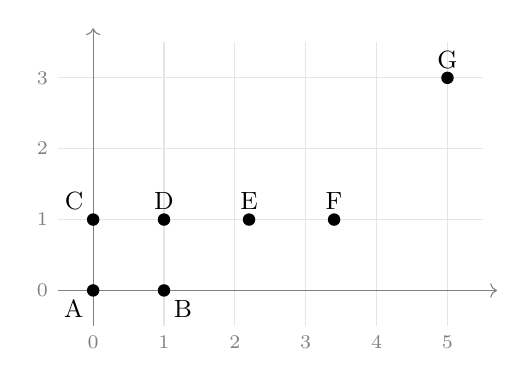
\begin{tikzpicture}[scale=0.9]
\draw[step=1,gray!20] (-0.5,-0.5) grid (5.5,3.5);
\draw[->,gray] (-0.5,0) -- (5.7,0);
\draw[->,gray] (0,-0.5) -- (0,3.7);
\foreach \x in {0,...,5} \node[below,font=\scriptsize,gray] at (\x,-0.5) {\x};
\foreach \y in {0,...,3} \node[left,font=\scriptsize,gray] at (-0.5,\y) {\y};
\foreach \p/\n/\pos in {{(0,0)}/A/below left,{(1,0)}/B/below right,{(0,1)}/C/above left,{(1,1)}/D/above,{(2.2,1)}/E/above,{(3.4,1)}/F/above,{(5,3)}/G/above}
  {\fill \p circle (2.5pt) node[\pos,font=\small] {\n};}
\end{tikzpicture}
\end{center}
Punktene er A$(0,0)$, B$(1,0)$, C$(0,1)$, D$(1,1)$, E$(2.2,1)$, F$(3.4,1)$ og G$(5,3)$.

Hvilken klassifisering av E, F og G er riktig?
\velg{Velg ett alternativ:}
\begin{alternativer}
\alt{A}{E, F og G er alle tre støypunkter}
\alt{B}{E og F er kantpunkter, mens G er støy}
\alt{C}{E er kjernepunkt, F er kantpunkt, G er støy}
\alt{D}{E er et kantpunkt, mens F og G er støy}
\end{alternativer}
\sporsmal{3}
Fire punkter i planet, $(0,0)$, $(0,4)$, $(6,0)$ og $(6,4)$, skal deles i to klynger. Vi sammenligner
inndelingen \emph{venstre/høyre} $\{(0,0),(0,4)\}$, $\{(6,0),(6,4)\}$ med inndelingen \emph{topp/bunn}
$\{(0,4),(6,4)\}$, $\{(0,0),(6,0)\}$. Begge bruker klyngegjennomsnittet som sentroide.

Hvilken inndeling har lavest verdi av størrelsen som \textbf{k-means minimerer}, og hva er verdien?
\velg{Velg ett alternativ:}
\begin{alternativer}
\alt{A}{Topp/bunn, med verdi 36}
\alt{B}{Venstre/høyre, med verdi 16}
\alt{C}{Venstre/høyre, med verdi 32}
\alt{D}{Topp/bunn, med verdi 72}
\end{alternativer}
\sporsmal{4}
En kollega kjører k-means for $k = 1,\dots,8$ og får inertia
\[
1000,\ 520,\ 300,\ 260,\ 230,\ 205,\ 185,\ 170 .
\]
Kollegaen vil velge $k = 8$ fordi inertia er lavest der.

Hvilket utsagn er riktig?
\velg{Velg ett alternativ:}
\begin{alternativer}
\alt{A}{Lavere inertia betyr mer kompakte klynger og dermed bedre clustering, så $k = 8$ er det riktige valget}
\alt{B}{Inertia sier lite om klyngekvalitet og bør derfor ikke brukes når $k$ velges, heller ikke sammen med andre metrikker}
\alt{C}{Inertia faller mest fra $k = 1$ til $k = 2$, og det største fallet angir riktig antall klynger, altså $k = 2$}
\alt{D}{Ved optimal plassering kan inertia aldri øke med $k$, så lavest inertia er ikke et gyldig kriterium for $k$}
\end{alternativer}
\makspoeng

\delstart{8}
\sporsmal{1}
Et t-SNE-plott av kundedata viser tre grupper: A er stor og spredt, B er liten og tett, og B og C
ligger nær hverandre, mens A ligger langt unna begge.

Hvilken konklusjon kan du trekke fra plottet?
\velg{Velg ett alternativ:}
\begin{alternativer}
\alt{A}{A er trolig mest spredt også i originalrommet, siden t-SNE bevarer variansen innen hver gruppe}
\alt{B}{Punkter som er nære naboer innen B i plottet, er trolig også nære naboer i originalrommet}
\alt{C}{B og C er trolig likere hverandre enn A, siden t-SNE bevarer avstandene mellom gruppene}
\alt{D}{B har trolig færrest punkter, siden arealet en gruppe dekker i plottet følger antall punkter}
\end{alternativer}
\sporsmal{2}
SNE lager en lavdimensjonal embedding av et datasett.

Hvilken beskrivelse av fremgangsmåten er riktig?
\velg{Velg ett alternativ:}
\begin{alternativer}
\alt{A}{Hovedkomponentene beregnes først og punktene projiseres på dem; deretter justeres $Q$ slik at variansen langs aksene blir størst mulig}
\alt{B}{$P$ beregnes i originalrommet, punktene plasseres tilfeldig i lav dimensjon og flyttes med gradient descent for å minimere $D_{KL}(P\|Q)$}
\alt{C}{$Q$ velges først i lav dimensjon, og deretter flyttes punktene i originalrommet med gradient descent til $P$ blir lik $Q$}
\alt{D}{Parvise avstander beregnes i originalrommet, og punktene plasseres i lav dimensjon slik at summen av kvadrerte avstandsavvik blir minst}
\end{alternativer}
\sporsmal{3}
En Isolation Forest med tre trær er tilpasset et datasett med 8 punkter. Tabellen viser dybden (antall
splitter fra rotnoden) der hvert punkt havner i en egen løvnode, i hvert av de tre trærne.
\begin{center}
\begin{tabular}{lcccccccc}
\toprule
Punkt & P1 & P2 & P3 & P4 & P5 & P6 & P7 & P8 \\
\midrule
Tre 1 & 9 & 2 & 8 & 5 & 10 & 3 & 7 & 2 \\
Tre 2 & 8 & 7 & 9 & 4 & 9 & 2 & 8 & 10 \\
Tre 3 & 10 & 3 & 7 & 6 & 11 & 4 & 9 & 9 \\
\bottomrule
\end{tabular}
\end{center}
Modellen skal markere de 25\,\% mest anomale punktene.

Hvilke punkter markeres som anomalier?
\velg{Velg ett alternativ:}
\begin{alternativer}
\alt{A}{P2 og P6}
\alt{B}{P1 og P5}
\alt{C}{P2 og P8}
\alt{D}{P2, P6 og P8}
\end{alternativer}
\sporsmal{4}
Du kjører PCA på de standardiserte featurene \emph{Høyde}, \emph{Vekt} og \emph{Alder} for en gruppe
voksne. Første hovedkomponent er enhetsvektoren
\[ \text{PC1} \approx (0.69,\ 0.70,\ 0.19) \quad \text{i rekkefølgen } (\textit{Høyde},\ \textit{Vekt},\ \textit{Alder}). \]
Person A får en stor positiv koordinat langs PC1.

Hva forteller dette mest sannsynlig om person A?
\velg{Velg ett alternativ:}
\begin{alternativer}
\alt{A}{A er først og fremst eldre enn snittet, siden PC1 forklarer mest av variansen i dataene}
\alt{B}{A er både høyere og tyngre enn snittet, mens alderen bidrar lite til koordinaten}
\alt{C}{A ligger omtrent like høyt over snittet i alle tre features, siden alle ladningene er positive}
\alt{D}{A har uvanlig stor spredning i egne målinger, siden PC1 er retningen med størst varians}
\end{alternativer}
\makspoeng

\delstart{9}
\sporsmal{1}
En agent trenes med $\epsilon$-greedy der $\epsilon$ starter på 1.0, ganges med en faktor litt under 1
etter hver episode, og aldri går under en minimumsverdi $\epsilon_{\min} = 0.01$.

Hvorfor er dette en fornuftig strategi?
\velg{Velg ett alternativ:}
\begin{alternativer}
\alt{A}{Q-verdiene er upålitelige tidlig, så da lønner utforsking seg mest; $\epsilon_{\min} > 0$ hindrer at agenten låser seg helt senere}
\alt{B}{Avtagende $\epsilon$ virker som en avtagende læringsrate, så Q-verdiene stabiliserer seg; $\epsilon_{\min} > 0$ hindrer at læringen stopper helt}
\alt{C}{Utforsking trengs bare til første belønning er funnet; $\epsilon_{\min} > 0$ brukes kun under trening og settes til 0 når agenten tas i bruk}
\alt{D}{Høy $\epsilon$ tidlig gjør at Q-verdiene oppdateres oftere, siden Q-tabellen bare oppdateres når en tilfeldig handling velges}
\end{alternativer}
\sporsmal{2}
I et rutenett-miljø har en agent funnet en vei til målet på 10 steg. Q-verdiene langs denne veien er
positive, mens alle andre Q-verdier fortsatt er 0. Ingen belønninger i miljøet er negative. Det finnes
også en kortere vei som agenten aldri har prøvd. Fra nå av settes $\epsilon = 0$.

Hva vil skje?
\velg{Velg ett alternativ:}
\begin{alternativer}
\alt{A}{Agenten følger den kjente veien og prøver aldri handlingene som fører mot den kortere veien}
\alt{B}{Agenten finner den kortere veien hvis læringsraten $\alpha$ økes, siden oppdateringene da blir større}
\alt{C}{Agenten finner etter hvert den kortere veien, fordi $\gamma < 1$ gir kortere veier høyere Q-verdi}
\alt{D}{Agenten utforsker maksimalt, siden $\epsilon = 0$ betyr at alle handlinger velges like ofte}
\end{alternativer}
\sporsmal{3}
En agent skal lære å spille et ballspill. Tilstanden agenten får, er ett enkelt bilde av spillet, som viser
hvor ballen er, men ikke hvilken vei eller hvor fort den beveger seg.

Er \textbf{Markov-egenskapen} oppfylt for denne tilstandsrepresentasjonen?
\velg{Velg ett alternativ:}
\begin{alternativer}
\alt{A}{Ja; så lenge belønningen bare avhenger av nåværende tilstand, er Markov-egenskapen oppfylt}
\alt{B}{Ja; Markov-egenskapen betyr bare at agenten ikke husker tidligere tilstander, og det gjelder her}
\alt{C}{Nei; neste tilstand avhenger også av fart og retning, som ett enkelt bilde ikke viser}
\alt{D}{Nei; Markov-egenskapen krever at miljøet er stokastisk, men ballens bevegelse er deterministisk}
\end{alternativer}
\sporsmal{4}
En MDP beskrives som $(S, A, P, R)$. Se på miljøet FrozenLake $4\times 4$ med \texttt{is\_slippery=False}:
agenten kan stå på 16 ruter, har 4 handlinger (venstre, ned, høyre, opp), og episoden avsluttes når
agenten faller i et hull eller når målet.

Hvilken beskrivelse av $P$ og $R$ er riktig?
\velg{Velg ett alternativ:}
\begin{alternativer}
\alt{A}{$P(S_{t+1}\mid S_t, A_t)$ er $1/4$ for hver naborute; $R$ er 1 ved mål og $-1$ ved fall i et hull}
\alt{B}{$P(S_{t+1}\mid S_t, A_t)$ er 1 for én bestemt neste tilstand; $R$ er 1 ved mål og ellers 0}
\alt{C}{$P(S_{t+1}\mid S_t, A_t)$ er $1/4$ for hver naborute; $R$ er 1 ved mål og ellers 0}
\alt{D}{$P(S_{t+1}\mid S_t, A_t)$ er 1 for én bestemt neste tilstand; $R$ er 1 ved mål og $-1$ ved fall i et hull}
\end{alternativer}
\makspoeng

\delstart{10}
\sporsmal{1}
Et SHAP force plot for én låntaker viser baseline $\phi_0 = 0.30$ (gjennomsnittsprediksjonen på
bakgrunnsdatasettet) og prediksjonen $f(\mathbf{x}^*) = 0.12$. Bidragene er
\begin{center}
\begin{tabular}{lcc}
\toprule
Feature & SHAP-verdi & Farge i plottet \\
\midrule
\emph{Alder} & $+0.05$ & rød \\
\emph{Inntekt} & $-0.15$ & blå \\
\emph{Gjeld} & $-0.08$ & blå \\
\bottomrule
\end{tabular}
\end{center}

Hvilket utsagn er riktig?
\velg{Velg ett alternativ:}
\begin{alternativer}
\alt{A}{Baseline 0.30 er prediksjonen modellen gir når alle featurene settes til 0}
\alt{B}{\emph{Alder} er rød fordi låntakeren har høy alder, siden fargen viser featurens verdi}
\alt{C}{For denne låntakeren er det \emph{Inntekt} som trekker prediksjonen lengst ned fra 0.30}
\alt{D}{\emph{Inntekt} er trolig den viktigste featuren for modellen generelt, siden den har størst $|\phi|$ her}
\end{alternativer}
\sporsmal{2}
Et team vil forklare én prediksjon fra et nevralt nettverk. De lager mange varianter av $\mathbf{x}^*$
ved å endre featureverdiene litt, lar nettverket predikere på dem, og tilpasser et \textbf{grunt
beslutningstre} til disse prediksjonene. Forklaringen de viser fram, er splittene i dette treet.

Hvilken av notatenes tre tilnærminger er dette?
\velg{Velg ett alternativ:}
\begin{alternativer}
\alt{A}{En surrogatmodell, der nettverket rundt $\mathbf{x}^*$ erstattes av en enklere, tolkbar funksjon}
\alt{B}{En tolkbar modell, siden det grunne treet erstatter nettverket når nye prediksjoner skal gjøres}
\alt{C}{SHAP, der input-featurene er spillere og prediksjonen fordeles mellom dem med Shapley-verdier}
\alt{D}{En modellspesifikk forklaring, der parametrene og strukturen i nettverket undersøkes direkte}
\end{alternativer}
\sporsmal{3}
Se på koden, der \texttt{history} kommer fra \texttt{model.fit(..., epochs=6, validation\_data=...)}:
\begin{lstlisting}[language=Python]
val_losses = history.history["val_loss"]
print(val_losses)   # [0.62, 0.48, 0.41, 0.43, 0.45, 0.47]
best_epoch = np.argmin(val_losses) + 1
print(best_epoch, val_losses[best_epoch])
\end{lstlisting}

Hva skriver den siste linjen ut?
\velg{Velg ett alternativ:}
\begin{alternativer}
\alt{A}{\texttt{2 0.41}}
\alt{B}{\texttt{6 0.47}}
\alt{C}{\texttt{3 0.43}}
\alt{D}{\texttt{3 0.41}}
\end{alternativer}
\sporsmal{4}
\texttt{X} har 1000 rader. Se på koden:
\begin{lstlisting}[language=Python]
X_tmp, X_test = train_test_split(X, test_size=0.2)
X_train, X_val = train_test_split(X_tmp, test_size=0.25)
print(len(X_train), len(X_val), len(X_test))
\end{lstlisting}

Hva skrives ut?
\velg{Velg ett alternativ:}
\begin{alternativer}
\alt{A}{\texttt{800 200 200}}
\alt{B}{\texttt{640 160 200}}
\alt{C}{\texttt{750 250 200}}
\alt{D}{\texttt{600 200 200}}
\end{alternativer}
\makspoeng

\clearpage
{\sffamily\bfseries\fontsize{18}{22}\selectfont Løsningsforslag}\par\vspace{0.3em}
\noindent\rule{\textwidth}{0.4pt}\par\vspace{1.2em}
Riktig alternativ per spørsmål (bokstaven står i rundingen foran hvert alternativ).\par\vspace{1em}
\begin{center}\sffamily\renewcommand{\arraystretch}{1.35}
\begin{tabular}{l*{4}{>{\centering\arraybackslash}p{1.6cm}}}
\toprule
& \textbf{Sp.\ 1} & \textbf{Sp.\ 2} & \textbf{Sp.\ 3} & \textbf{Sp.\ 4}\\
\midrule
Part 1 & B & C & C & B\\
Part 2 & A & D & C & B\\
Part 3 & D & D & A & D\\
Part 4 & C & D & D & B\\
Part 5 & B & A & C & C\\
Part 6 & A & D & C & A\\
Part 7 & A & D & B & D\\
Part 8 & B & B & A & B\\
Part 9 & A & A & C & B\\
Part 10 & C & A & C & D\\
\bottomrule
\end{tabular}
\end{center}
\end{document}
